% Paquets généraux
\documentclass[a4paper,12pt,titlepage]{article}
\usepackage[T1]{fontenc}
\usepackage[utf8]{inputenc}
\usepackage[french]{babel}
\usepackage[gen]{eurosym}
%\usepackage[dvips]{graphicx}
\usepackage{fancyhdr}
\usepackage{pdfpages} 
\usepackage{multido}
\usepackage{hyperref}
%\usepackage{textcomp}
%\usepackage{aeguill}
\usepackage{schemabloc}
\usepackage[bitstream-charter]{mathdesign}

\newcommand{\id}{54}
\newcommand{\nom}{Liaisons mécaniques}
\newcommand{\sequence}{04}
\newcommand{\num}{01}
\newcommand{\type}{TP}
\newcommand{\descrip}{Modélisation d'un solide. Comportement des liaisons mécaniques. Modéliser les mécanismes du laboratoire par un schéma cinématique, paramétré.}
\newcommand{\competences}{A3-C4: Analyse d'architecture et de comportement \\ &  Mod1-C1: Isolement d'un solide ou d'un système de solides \\ &  Mod2-C10-1: Modèle de solide indéformable \\ &  Mod2-C11: Modélisation géométrique et cinématique des mouvements entre solides indéformables \\ &  Mod2-C12: Modélisation cinématique des liaisons entre solides \\ &  Mod2-C15: Modélisation des actions mécaniques \\ &  Rés-C6: Utilisation d'un solveur ou d'un logiciel multi physique \\ &  Com1-C1: Différents descripteurs introduits dans le programme \\ &  Com2-C4: Outils de communication}
\newcommand{\nbcomp}{9}
\newcommand{\systemes}{Plateforme Stewart}
\newcommand{\systemessansaccent}{Plateforme Stewart}
\newcommand{\ilot}{2}
\newcommand{\ilotstr}{02}
\newcommand{\dossierilot}{\detokenize{Ilot_02 Plateforme Stewart}}
\newcommand{\imageun}{Plateforme}

\newcommand{\urlsysteme}{\href{https://www.costadoat.fr/systeme/57}{Ressources système}}
\newcommand{\matlabsimscape}{\href{https://github.com/Costadoat/Sciences-Ingenieur/raw/master/Systemes/Plateforme Stewart/Plateforme_Stewart_Simscape.zip}{Modèle Simscape}}
\newcommand{\solidworks}{\href{https://github.com/Costadoat/Sciences-Ingenieur/raw/master/Systemes/Plateforme Stewart/Plateforme_Stewart_Solidworks.zip}{Modèle Solidworks}}
\newcommand{\edrawings}{\href{https://github.com/Costadoat/Sciences-Ingenieur/raw/master/Systemes/Plateforme Stewart/Plateforme_Stewart.EASM}{Modèle eDrawings}}
\newcommand{\test}{Stewart_param1}
\newcommand{\testi}{Stewart_param2}
\newcommand{\testii}{Stewart_param3}
\newcommand{\testiii}{Stewart_param4}
\newcommand{\testiiii}{Stewart_euler}

\newcommand{\auteurun}{Renaud Costadoat}
\newcommand{\auteurdeux}{Françoise Puig}
\newcommand{\institute}{Lycée Dorian}


\usepackage{color}
\usepackage{xcolor}
\usepackage{colortbl}
\usepackage{helvet}
\renewcommand{\familydefault}{\sfdefault}
\usepackage{amsfonts}
\usepackage{amsmath}
%\usepackage{xspace}
\usepackage{varioref}
\usepackage{tabularx}
%\usepackage{floatflt}
\usepackage{graphics}
\usepackage{wrapfig}
\usepackage{textcomp}
\usepackage{tikz}
\usepackage{wrapfig}
\usepackage{gensymb}
\usepackage[european]{circuitikz}
\usetikzlibrary{babel}
\usepackage{ifthen}
\usepackage{cancel}
\usepackage{etoolbox}
\usepackage{multirow}
%\usepackage{boxedminipage}
\definecolor{gris25}{gray}{0.75}
\definecolor{bleu}{RGB}{18,33,98}
\definecolor{bleuf}{RGB}{42,94,171}
\definecolor{bleuc}{RGB}{231,239,247}
\definecolor{rougef}{RGB}{185,18,27}
\definecolor{rougec}{RGB}{255,188,204}%255,230,231
\definecolor{vertf}{RGB}{103,126,82}
\definecolor{vertc}{RGB}{220,255,191}
\definecolor{forestgreen}{rgb}{0.13,0.54,0.13}
\definecolor{blcr}{rgb}{0.59,0.69,0.84}
\definecolor{blfr}{rgb}{0.32,0.51,0.75}
\definecolor{orfr}{rgb}{0.90,0.42,0.15}
\definecolor{orcr}{rgb}{0.90,0.65,0.50}
\definecolor{orangef}{rgb}{0.659,0.269,0.072}
\definecolor{orange}{rgb}{0.58,0.35,0.063}
\definecolor{orangec}{rgb}{0.43,0.32,0.25}
\definecolor{rcorrect}{rgb}{0.6,0,0}
\definecolor{sequence}{rgb}{0.75,0.75,0.75}
\definecolor{competences}{rgb}{0.61,0.73,0.35}
\definecolor{grisf}{HTML}{222222}
\definecolor{grisc}{HTML}{636363}
\definecolor{normal}{HTML}{4087c4}
\definecolor{info}{HTML}{5bc0de}
\definecolor{success}{RGB}{92,184,92}
\definecolor{warning}{RGB}{240,173,78}
\definecolor{danger}{RGB}{217,83,79}
\hypersetup{                    % parametrage des hyperliens
    colorlinks=true,                % colorise les liens
    breaklinks=true,                % permet les retours à la ligne pour les liens trop longs
    urlcolor= blfr,                 % couleur des hyperliens
    linkcolor= orange,                % couleur des liens internes aux documents (index, figures, tableaux, equations,...)
    citecolor= forestgreen                % couleur des liens vers les references bibliographiques
    }

% Mise en page
\pagestyle{fancy}

\setlength{\hoffset}{-18pt}

\setlength{\oddsidemargin}{0pt} 	% Marge gauche sur pages impaires
\setlength{\evensidemargin}{0pt} 	% Marge gauche sur pages paires
\setlength{\marginparwidth}{00pt} 	% Largeur de note dans la marge
\setlength{\headwidth}{481pt} 	 	% Largeur de la zone de tête (17cm)
\setlength{\textwidth}{481pt} 	 	% Largeur de la zone de texte (17cm)
\setlength{\voffset}{-18pt} 		% Bon pour DOS
\setlength{\marginparsep}{7pt}	 	% Séparation de la marge
\setlength{\topmargin}{-30pt} 		% Pas de marge en haut
\setlength{\headheight}{35pt} 		% Haut de page
\setlength{\headsep}{20pt} 		% Entre le haut de page et le texte
\setlength{\footskip}{30pt} 		% Bas de page + séparation
\setlength{\textheight}{700pt} 		% Hauteur de l'icone zone de texte (25cm)
\setlength\fboxrule{1 pt}
\renewcommand{\baselinestretch}{1}
\setcounter{tocdepth}{1}
\newcommand{\cadre}[2]
{\fbox{
  \begin{minipage}{#1\linewidth}
   \begin{center}
    #2\\
   \end{center}
  \end{minipage}
 }
}

\newcounter{num_quest} \setcounter{num_quest}{0}
\newcounter{num_rep} \setcounter{num_rep}{0}
\newcounter{num_cor} \setcounter{num_cor}{0}

\newcommand{\question}[1]{\refstepcounter{num_quest}\par
~\ \\ \parbox[t][][t]{0.15\linewidth}{\textbf{Question \arabic{num_quest}}}\parbox[t][][t]{0.93\linewidth}{#1}\par
}


\newcommand{\reponse}[1]
{\refstepcounter{num_rep}
\noindent
\rule{\linewidth}{.5pt}
\textbf{Question \arabic{num_rep}:}
\multido{\i=1+1}{#1}{~\ \\}
}

\newcommand{\cor}
{\refstepcounter{num_cor}
\noindent
\rule{\linewidth}{.5pt}
\textbf{Question \arabic{num_cor}:} \\
}

\newcommand{\titre}[1]
{\begin{center}
\cadre{0.8}{\huge #1} 
\end{center}
}


% En tête et pied de page
\fancypagestyle{normal}{%
  \fancyhf{}
\lhead{\nom}
\rhead{
\includegraphics[width=2cm]{../../img/logo}\hspace{2pt}}
\ifdef{\auteurdeux}{\lfoot{\auteurun,\auteurdeux}}{\lfoot{\auteurun}}
\cfoot{Page \thepage}}

\fancypagestyle{correction}{%
  \fancyhf{}
  \lhead{\colorbox{danger}{\begin{minipage}{0.65\paperwidth} \textcolor{white}{\textbf{Correction}} \end{minipage}} }
  \rhead{
\includegraphics[width=2cm]{../../img/logo}}
  \ifdef{\auteurdeux}{\lfoot{\auteurun,\auteurdeux}}{\lfoot{\auteurun}}
  \rfoot{\colorbox{danger}{\begin{minipage}{0.5\paperwidth} \begin{flushright}\textcolor{white}{\textbf{Correction}}\end{flushright} \end{minipage}} }}

\renewcommand{\footrulewidth}{0.4pt}

\usepackage{eso-pic}
\newcommand{\BackgroundPic}{%
\put(0,0){%
\parbox[b][\paperheight]{\paperwidth}{%
\vfill
\begin{center}
\hspace{0.5cm}\vspace{0.5cm}

\includegraphics[width=\paperwidth,height=\paperheight,%
keepaspectratio]{../../img/fond3}%
\end{center}
\vfill
}}}

\newcommand{\BackgroundPicdeux}{%
\put(25,-30){%
\parbox[b][\paperheight]{\paperwidth}{%
\vfill
\begin{center}

\includegraphics[width=\paperwidth,height=\paperheight,%
keepaspectratio]{../../img/fond4}%
\end{center}
\vfill
}}}

\begin{document}

\pagestyle{empty}

\vspace*{-3\baselineskip}

\AddToShipoutPicture*{\BackgroundPic}

\ifdef{\auteurdeux}{\begin{tabular}{>{\columncolor{gray!00}}m{.3\linewidth} m{.3\linewidth} >{\columncolor{gray!00}}m{.3\linewidth}}
Séquence : \sequence &  \multirow{3}{*}{\hspace{1cm}
\includegraphics[height=1.5cm]{../../img/logo}} &  \begin{flushright} \multirow{4}{*}{\hspace{1cm}
\includegraphics[height=4cm]{img/qrcode}}\end{flushright}\\
Document : \type\num \\
 \institute \\
 \auteurun\\
 \auteurdeux
\end{tabular}}{\begin{tabular}{>{\columncolor{gray!00}}m{.3\linewidth} m{.3\linewidth} >{\columncolor{gray!00}}m{.3\linewidth}}
Séquence : \sequence &  \multirow{3}{*}{\hspace{1cm}
\includegraphics[height=1.5cm]{../../img/logo}} &  \begin{flushright} \multirow{4}{*}{\hspace{1cm}
\includegraphics[height=4cm]{img/qrcode}}\end{flushright}\\
Document : \type\num \\
 \institute \\
 \auteurun
\end{tabular}}

\vspace{1cm}

\ifdef{\prive}{\begin{center}\colorbox{danger}{\Huge{Avec Correction}}\end{center}}{}

\begin{center}\huge{\nom}\end{center}

\vspace{2cm}

\ifdef{\imagedeux}{\begin{minipage}{0.49\linewidth}}{}
\begin{center}\includegraphics[height=5cm]{/home/renaud/Documents/Renaud/GitHub/django_education/systemes/\imageun}\end{center}
\ifdef{\imagedeux}{\end{minipage}\hfill
\begin{minipage}{0.49\linewidth}
\begin{center}\includegraphics[height=5cm]{/home/renaud/Documents/Renaud/GitHub/django_education/systemes/\imagedeux}\end{center}
\end{minipage}}{}

\vspace{5cm}


\begin{tabular}{p{.15\linewidth} >{\columncolor{white}}p{.8\linewidth}}
    \rowcolor{gray!20}
    Référence & S\sequence\ - \type\num \\
    Compétences & \competences \\
 	\rowcolor{gray!20}
    Description & \descrip \\
    Système & \systemes
  \end{tabular}

\newpage

\AddToShipoutPicture{\BackgroundPicdeux}

\pagestyle{normal}

\section{Rappels}

\subsection{Les bases du calcul vectoriel}

Soit le vecteur $\overrightarrow{u}=\left(\begin{tabular}{c} 8 \\ 5 \\ 4 \end{tabular}\right)$.

\paragraph{Question 1:} Calculer sa norme.

\vspace{10pt}

On donne le vecteur $\overrightarrow{v}=\left(\begin{tabular}{c} 6 \\ y \\ z \end{tabular}\right)$.

\paragraph{Question 2:} Trouver y et z tels que les deux vecteurs soient colinéaires. Montrer que deux méthodes sont possibles mais vous en choisirez une seule pour la démonstration.

\subsection{Produit scalaire}

Soient deux vecteurs $\overrightarrow{u}=\left(\begin{tabular}{c} 18 \\ 7 \\ 13 \end{tabular}\right)$ et $\overrightarrow{v}=\left(\begin{tabular}{c} 23 \\ -54 \\ 36 \end{tabular}\right)$.

\paragraph{Question 1:} Calculer les normes de ces vecteurs.

\paragraph{Question 2:} Calculer le produit scalaire de ces vecteurs.

\paragraph{Question 3:} A partir des résultats précédents, calculer l'angle entre les deux vecteurs.

\subsection{Produit vectoriel}

Soient deux vecteurs $\overrightarrow{u}=\left(\begin{tabular}{c} 2 \\ 3 \\ 6 \end{tabular}\right)$ et $\overrightarrow{v}=\left(\begin{tabular}{c} 1 \\ 5 \\ 2 \end{tabular}\right)$.

\paragraph{Question 1:} Calculer les normes de ces vecteurs.

\paragraph{Question 2:} Calculer le produit vectoriel de ces vecteurs.

\paragraph{Question 3:} A partir des résultats précédents, calculer l'angle entre les deux vecteurs.

\newpage

\section{Étude géométrique machine de dépose joint liquide}

\subsection{Mise en situation}

La société John Deere conçoit et fabrique du matériel agricole. L'usine, située dans le Loiret, est chargée de la fabrication et du montage des moteurs Diesel de 3, 4, ou 6 cylindres.
Les photos de la figure \ref{fig:image1} montrent la chaîne d'assemblage des moteurs, ceux-ci étant maintenus sur des balancelles.
La pièce qui a pour fonction principale de collecter les gaz d'échappement issus des cylindres pour les envoyer vers le pot d'échappement s'appelle le collecteur d'échappement.
Le sujet a pour thème l'étude du poste de dépose du joint liquide sur le collecteur d'échappement du moteur.


\begin{figure}[htbp]
\begin{center}
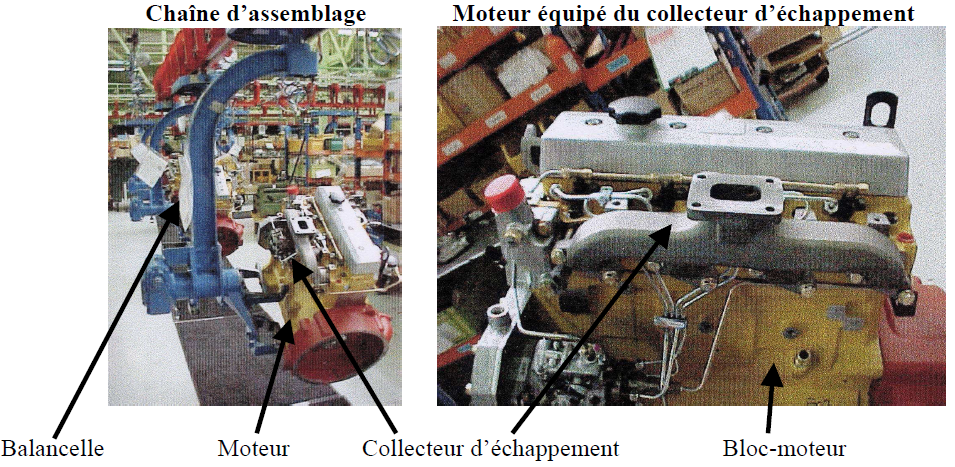
\includegraphics[width=0.7\linewidth]{img/Image2.png}
\caption{Chaîne de fabrication}
\label{fig:image1}
\end{center}
\end{figure}

\subsection{Présentation du système}

\begin{figure}[htbp]
\begin{minipage}[c]{.35\linewidth}
\begin{center}
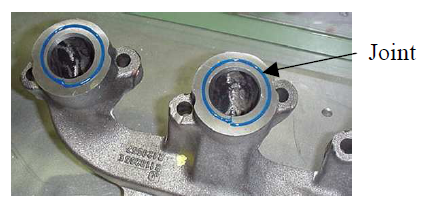
\includegraphics[width=\linewidth]{img/Image35.png}
\caption{Joints déposés}
\label{fig:image2}
\end{center}
\end{minipage}
\hfill
\begin{minipage}[c]{.62\linewidth}
Initialement, l'étanchéité aux gaz d'échappement entre le moteur et le collecteur d'échappement était réalisée par des joints métalliques. Leur mise en place était compliquée, l'étanchéité n'était pas optimale.
C'est pourquoi, après plusieurs essais, la société John Deere a souhaité appliquer un nouveau procédé d'étanchéité réalisé par la dépose d'un joint liquide effectué sur une machine de dépose automatisée.
Ces joints sont 10 fois moins onéreux, sont plus efficaces, et nécessitent une moins bonne qualité de surface des zones de contact entre moteur et collecteur, figure \ref{fig:image1} et \ref{fig:image2}.
\end{minipage}
\end{figure}

\newpage

\subsection{Analyse géométrique du robot}

L'étude va porter sur le moment où le robot se déplace vers le premier trou (pige commune rouge et coordonnées connues et identiques quel que soit le type de collecteur).
C'est l'action : déplacer robot trajectoire 1, présentée à la figure  \ref{fig:image25}.

\begin{figure}[htbp]
\begin{center}
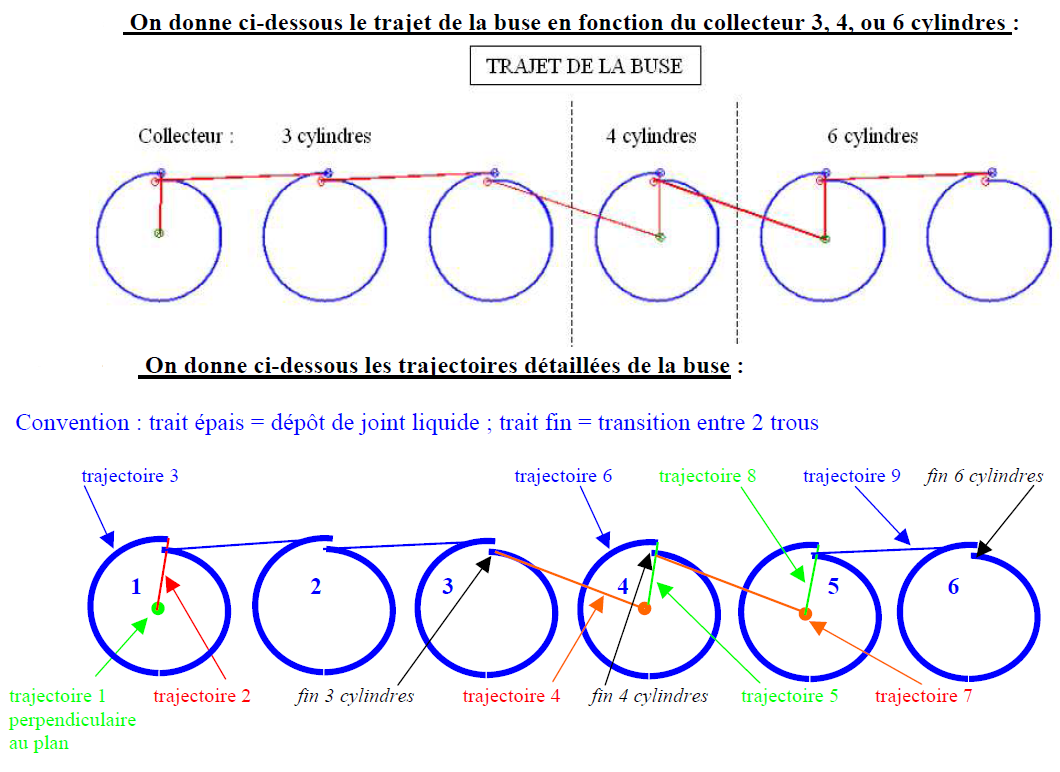
\includegraphics[width=0.6\linewidth]{img/Image8.png}
\caption{Trajectoire 1}
\label{fig:image25}
\end{center}
\end{figure}

Deux vues du robot ABB, dont le bras supporte la buse de dépose du joint liquide, sont représentées sur les figures \ref{fig:image3} et \ref{fig:image4} :
\begin{itemize}
 \item Vue de face,
 \item Vue de dessus.
\end{itemize}

Dans ces 2 vues, on a représenté le robot avec : $\theta_{01}=\theta_{34}=\theta_{45}=\theta_{56}=0$\textdegree et $\theta_{12}=-\theta_{23}$ 
\paragraph{Question 1 :} Pourquoi on nomme un tel robot, un robot 6 axes.


\begin{figure}[htbp]
\begin{minipage}[c]{.48\linewidth}
\begin{center}
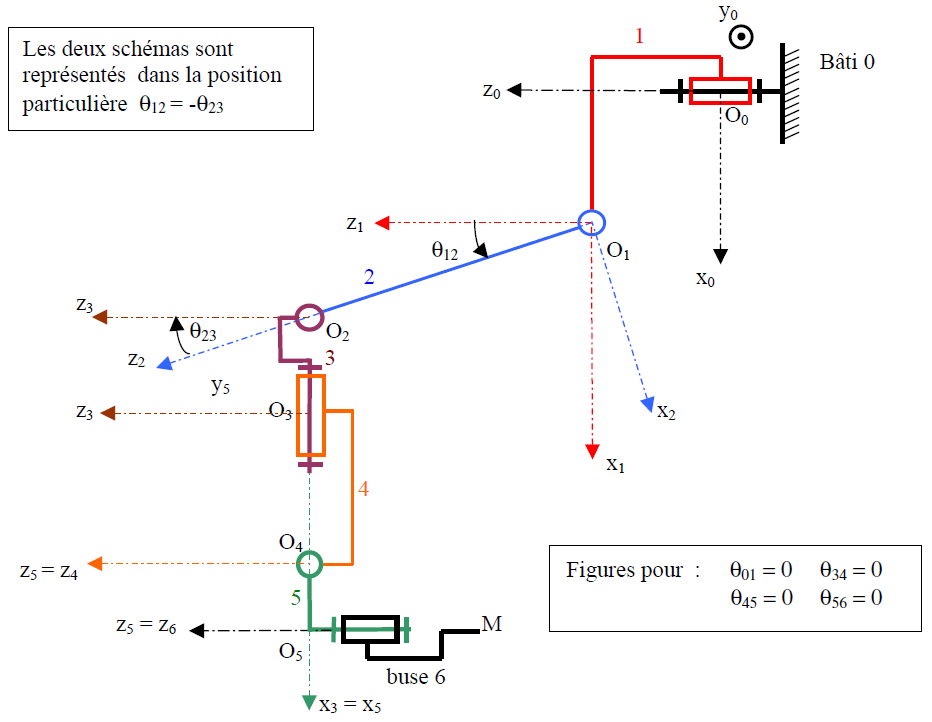
\includegraphics[width=\linewidth]{img/Image5.png}
\caption{Schéma cinématique 1}
\label{fig:image3}
\end{center}
\end{minipage}
\hfill
\begin{minipage}[c]{.48\linewidth}
\begin{center}
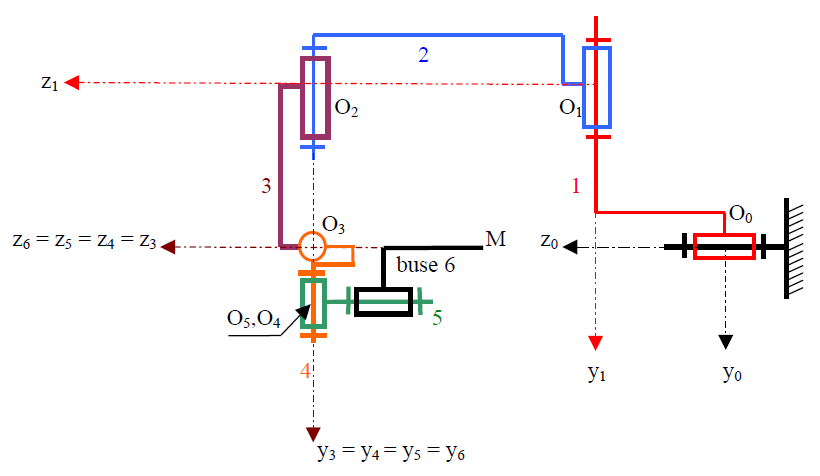
\includegraphics[width=\linewidth]{img/Image6.png}
\caption{Schéma cinématique 2}
\label{fig:image4}
\end{center}
\end{minipage}
\end{figure}

\newpage

La figure \ref{fig:image5} présente le robot en position \og parking \fg :
$\theta_{01}=-90$\textdegree, $\theta_{12}=14$\textdegree et $\theta_{23}=-14$\textdegree


\begin{figure}[htbp]
\begin{minipage}[c]{.4\linewidth}
\begin{center}
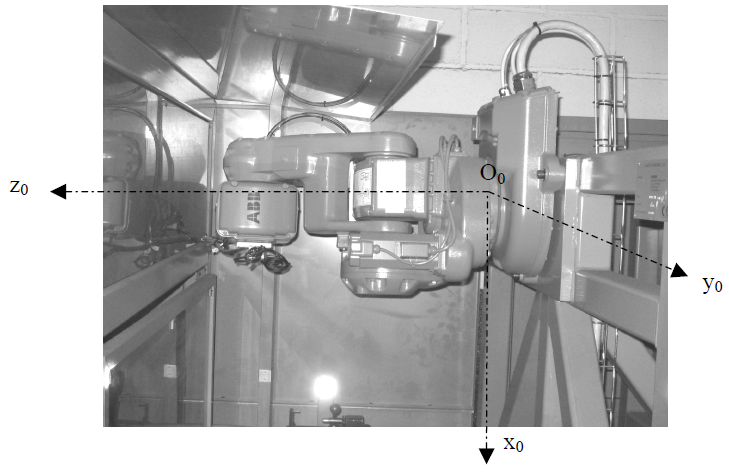
\includegraphics[width=\linewidth]{img/Image1.png}
\caption{Bras en position parking}
\label{fig:image5}
\end{center}
\end{minipage}
\hfill
\begin{minipage}[c]{.55\linewidth}
Détermination du premier point de la trajectoire 1

On se propose de déterminer les coordonnées du premier point de la trajectoire de l'extrémité de la buse M dans $R_0(O,\overrightarrow{x_0},\overrightarrow{y_0},\overrightarrow{z_0})$ :, au début du mouvement de translation défini lors de la trajectoire 1. C'est le premier point que le point M, extrémité de la buse, devra rejoindre au début du programme de dépose du joint liquide.
Le schéma cinématique donné sur les figures \ref{fig:image3} et \ref{fig:image4} a été effectué pour :

$\theta_{01}=\theta_{34}=\theta_{45}=\theta_{56}=0$\textdegree et $\theta_{12}=-\theta_{23}$ 
\end{minipage}
\end{figure}

On donne le paramétrage et les figures de calcul:

Paramétrage :

\begin{figure}[htbp]
 \begin{tabular}{l l l l}
 $\overrightarrow{O_{0}O_1}=a.\overrightarrow{x_1}+b.\overrightarrow{z_0}-f.\overrightarrow{y_1}$ &
 $\overrightarrow{O_{1}O_2}=c.\overrightarrow{z_2}$ &
 $\theta_{01}=\left(\overrightarrow{x_0},\overrightarrow{x_1}\right)$ &
 $\theta_{12}=\left(\overrightarrow{x_1},\overrightarrow{x_2}\right)$ \\
 $\overrightarrow{O_{2}O_3}=d.\overrightarrow{x_3}+f.\overrightarrow{y_3}$ &
 $\overrightarrow{O_{3}O_4}=e.\overrightarrow{x_3}+h.\overrightarrow{y_4}$ &
 $\theta_{23}=\left(\overrightarrow{x_2},\overrightarrow{x_3}\right)$ &
 $\theta_{34}=\left(\overrightarrow{y_3},\overrightarrow{y_4}\right)$ \\
 $\overrightarrow{O_{4}O_5}=g.\overrightarrow{x_5}$ &
 $\overrightarrow{O_{5}M}=-h.\overrightarrow{y_6}-l.\overrightarrow{z_6}$ &
 $\theta_{45}=\left(\overrightarrow{z_4},\overrightarrow{z_5}\right)$ &
 $\theta_{56}=\left(\overrightarrow{y_5},\overrightarrow{y_6}\right)$
 \end{tabular}
\end{figure}

\begin{figure}[htbp]
\begin{center}
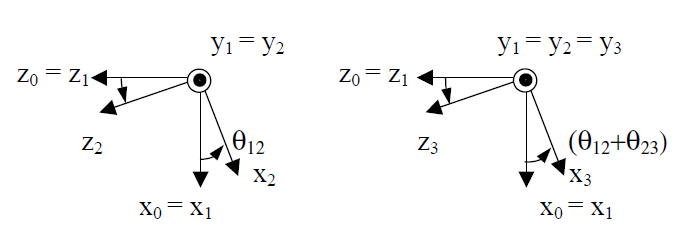
\includegraphics[width=0.5\linewidth]{img/Image7.png}
\caption{Figures de calcul}
\label{fig:image6}
\end{center}
\end{figure}

Dans la position particulière du premier point de la trajectoire 1 de la buse, on a les angles suivants :
$\theta_{01}=\theta_{34}=\theta_{45}=\theta_{56}=0$\textdegree.

\paragraph{Question 2:}

Déterminer pour la position particulière définie ci-dessus, en fonction du paramétrage donné, les vecteurs suivants :

\begin{itemize}
 \item $\overrightarrow{O_{0}O_1}$ en projection sur les axes $\left(\overrightarrow{x_0},\overrightarrow{y_0},\overrightarrow{z_0}\right)$,
  \item $\overrightarrow{O_{1}O_2}$ en projection sur l'axe $\left(\overrightarrow{z_2}\right)$,
 \item $\overrightarrow{O_{2}O_3}$ en projection sur les axes $\left(\overrightarrow{x_3},\overrightarrow{y_0}\right)$,
 \item $\overrightarrow{O_{3}O_4}$ en projection sur les axes $\left(\overrightarrow{x_3},\overrightarrow{y_0}\right)$,
 \item $\overrightarrow{O_{4}O_5}$ en projection sur l'axe $\left(\overrightarrow{x_3}\right)$,
 \item $\overrightarrow{O_{5}M}$ en projection sur les axes $\left(\overrightarrow{y_0},\overrightarrow{z_3}\right)$,
\end{itemize}

\paragraph{Question 3:}

Déterminer pour la position particulière définie ci-dessus, en fonction du paramétrage donné, le vecteur suivant :

\begin{itemize}
 \item $\overrightarrow{O_{0}M}$ en projection sur les axes $\left(\overrightarrow{x_0},\overrightarrow{y_0},\overrightarrow{z_0}\right)$.
\end{itemize}

\newpage

\section{La chaise de dentiste: Bac STI (GE) 2006}

\subsection{Mise en situation}

\begin{figure}[htbp]
\begin{minipage}[c]{.4\linewidth}
\begin{center}
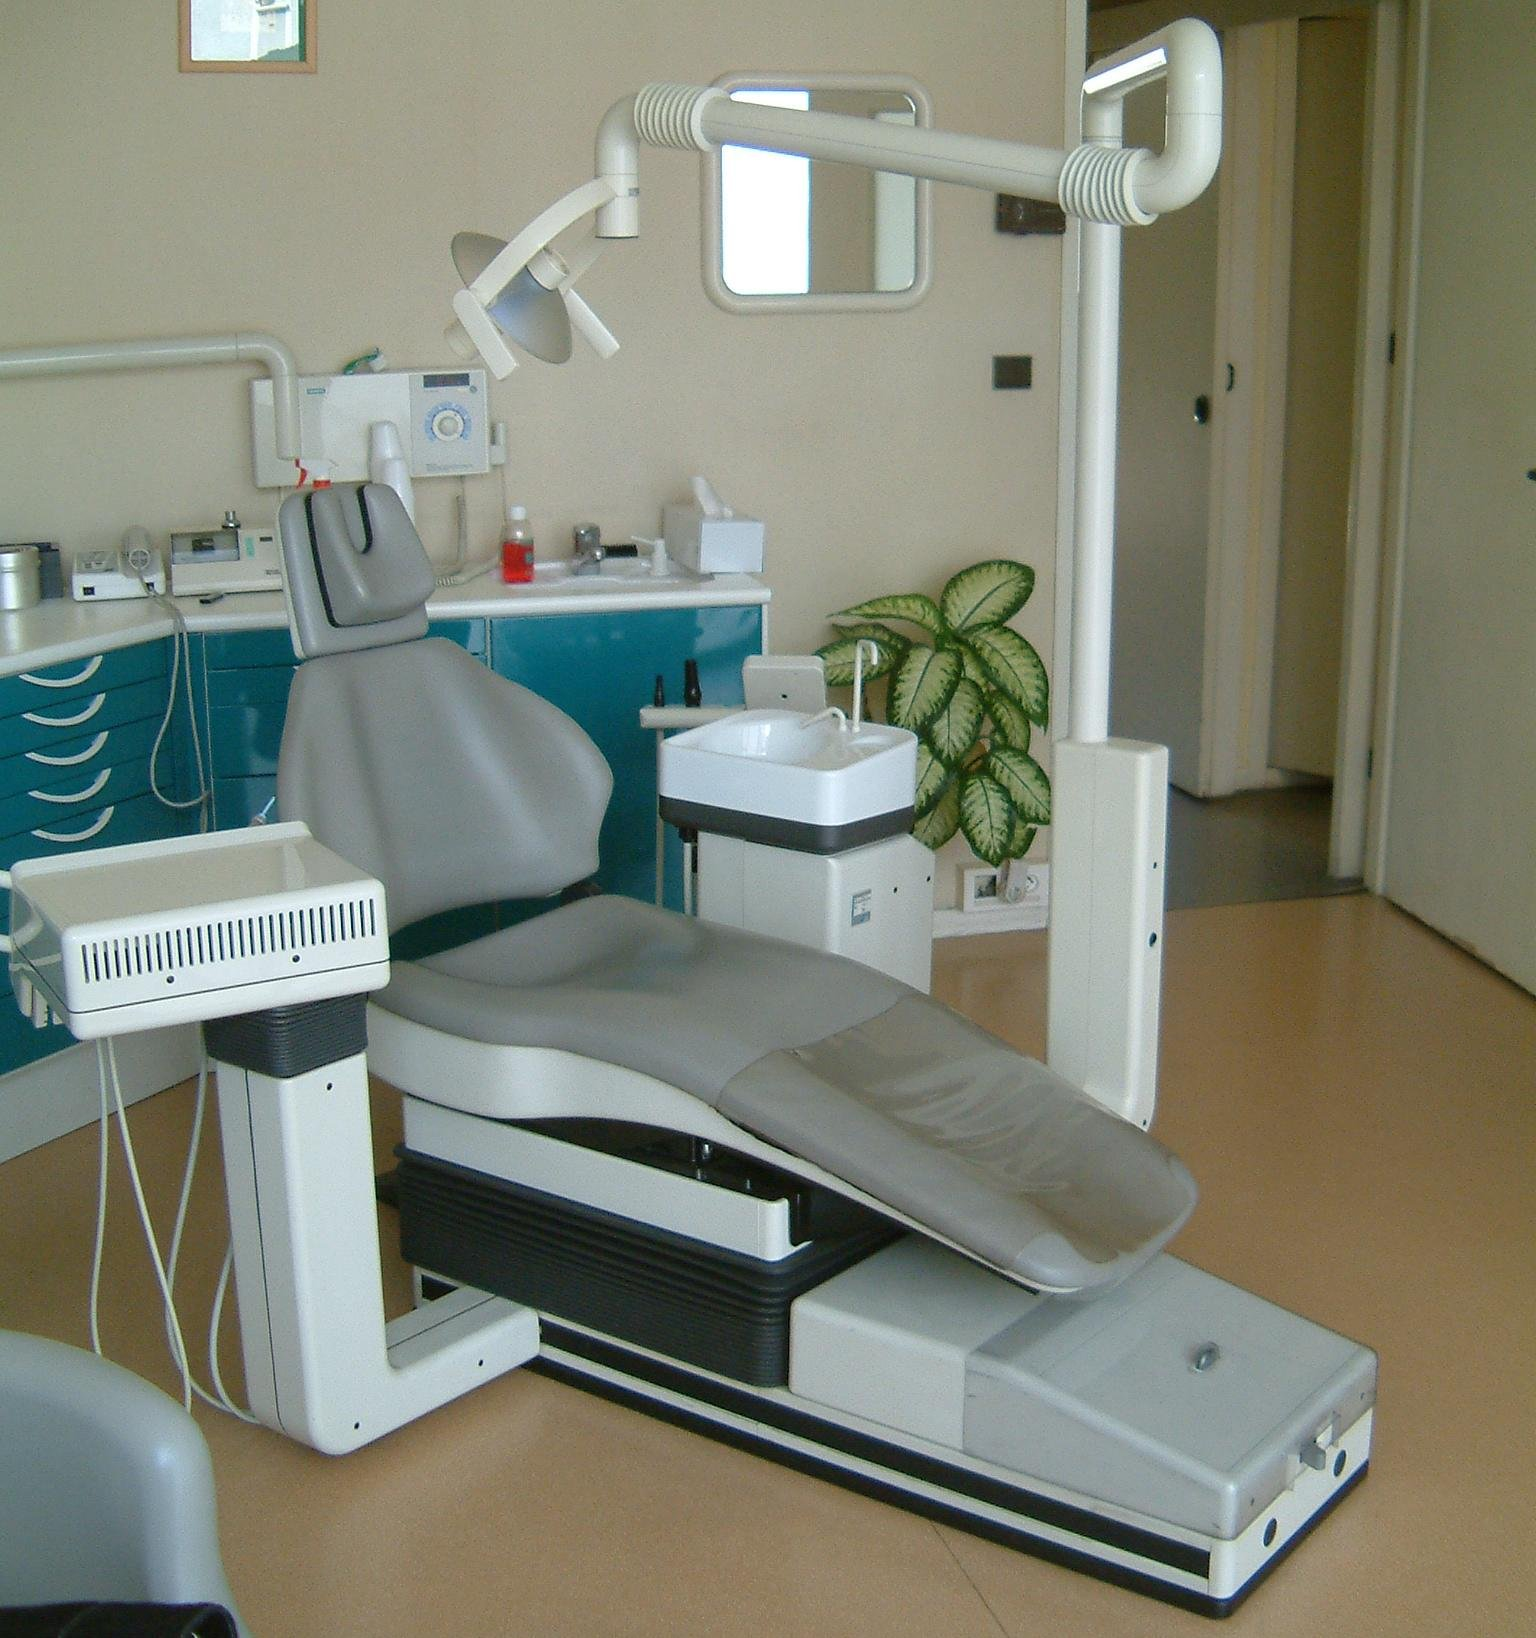
\includegraphics[width=\linewidth]{img/cabinet.jpg}
\caption{Fauteuil dans un cabinet}
\label{fig:imagechaise1}
\end{center}
\end{minipage}
\hfill
\begin{minipage}[c]{.55\linewidth}
La chirurgie dentaire et ses spécificités opératoires nécessitent l'installation du patient dans une position couchée particulière (voir illustration ci-dessous). La société AIREL a donc développé un fauteuil d'opération ergonomique, véritable automate comportant toutes les commandes et les fonctions dont le praticien doit disposer, quelle que soit sa spécialité et ses contraintes opératoires.
\end{minipage}
\end{figure}

\subsection{Présentation du système}

\begin{figure}[htbp]
\begin{minipage}[c]{.5\linewidth}
Le système de levée du fauteuil, qui va être l'objet de notre étude, est composé d'un vérin ainsi que d'un système pantographe.

Il permet de piloter la montée et la descente du fauteuil afin de placer le patient à une hauteur adéquate afin que le médecin pratique son intervention dans les meilleures conditions possibles.
\end{minipage}
\hfill
\begin{minipage}[c]{.45\linewidth}
\begin{center}
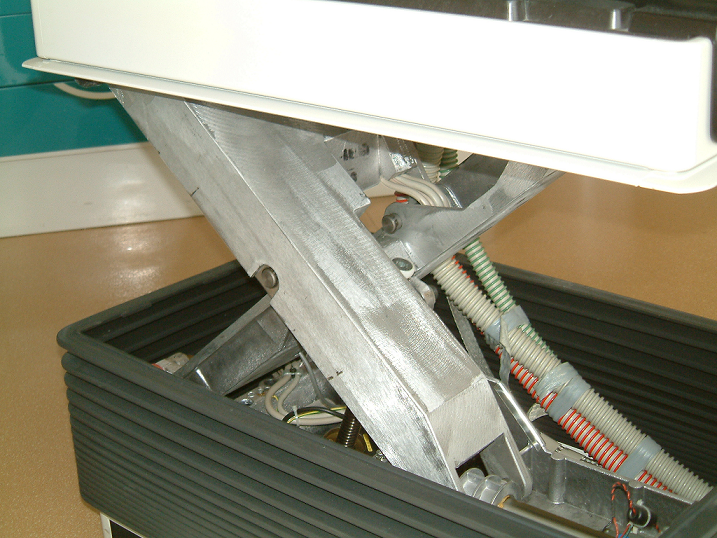
\includegraphics[width=\linewidth]{img/detail_chaise.png}
\caption{Système de levée}
\label{fig:imagechaise2}
\end{center}
\end{minipage}
\end{figure}

\newpage

\subsection{Descriptif de la géométrie}

La figure \ref{fig:imagechaise7}, montre les pièces du système numérotées.

\begin{itemize}
 \item $\overrightarrow{AD}=a.\overrightarrow{x}+b.\overrightarrow{y}$,
 \item $\overrightarrow{DK}=2.\overrightarrow{DC}=2.c.\overrightarrow{x_3}$,
 \item $\overrightarrow{DB}=d.\overrightarrow{x_3}+e.\overrightarrow{y_3}$,
 \item $\overrightarrow{AB}=l_1.\overrightarrow{x_6}$,
 \item $\overrightarrow{HE}=2.\overrightarrow{HC}=2.c.\overrightarrow{x_4}$.
\end{itemize}

~\

La construction géométrique du système \og 4 barres \fg permet de dire que:
\begin{itemize}
 \item $\overrightarrow{DE}=\overrightarrow{HK}=l_2.\overrightarrow{y}$,
 \item $\overrightarrow{HD}=\overrightarrow{KE}=l_3.\overrightarrow{x}$,
\end{itemize}

~\

Les distances $a$,$b$,$c$,$d$ et $e$ sont fixées par les dimensions du mécanisme. Les longueurs $l_1$, $l_2$ et $l_3$ sont variables.
 
\begin{figure}[htbp]
\begin{center}
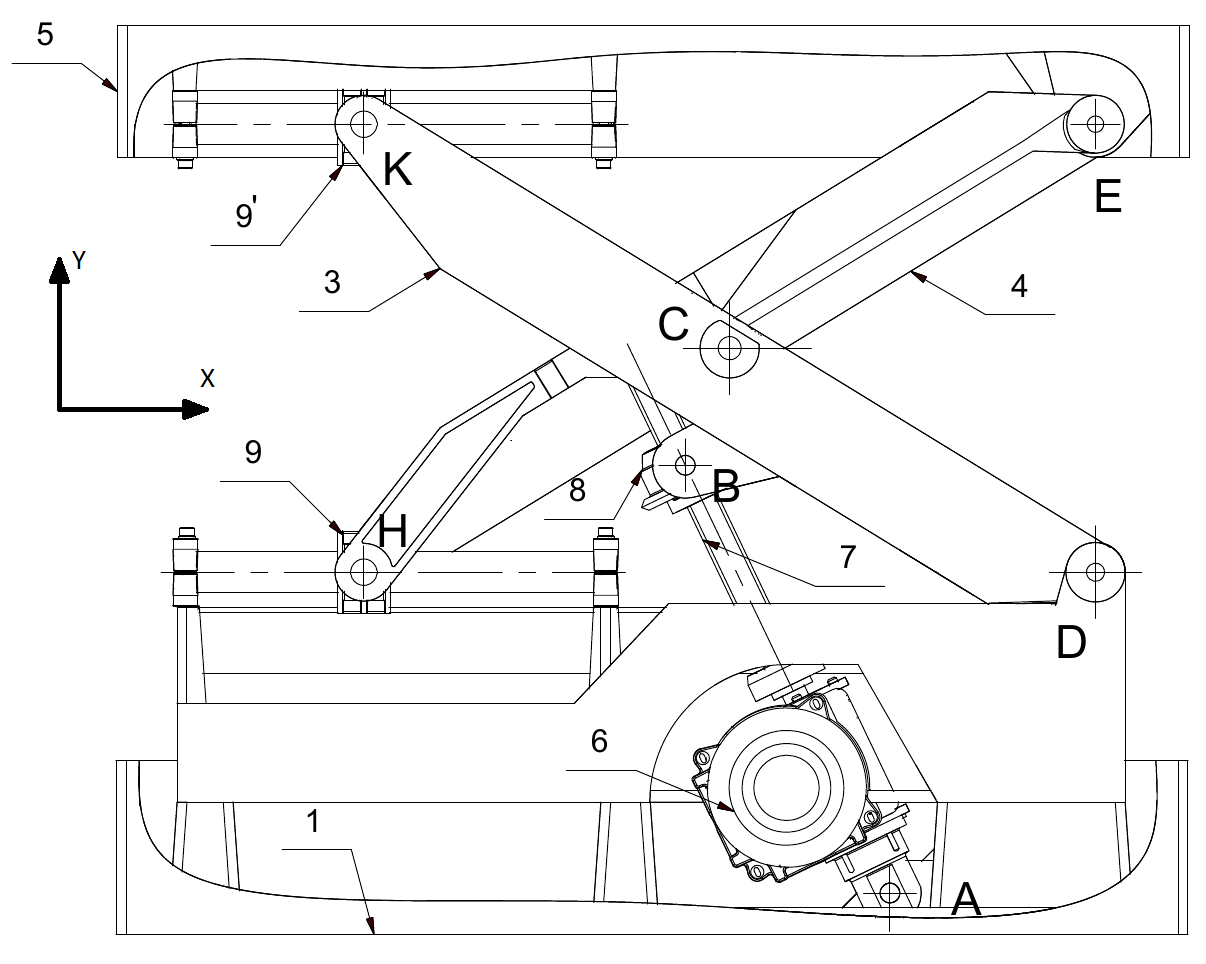
\includegraphics[width=\linewidth]{img/face.png}
\caption{Système de levée}
\label{fig:imagechaise7}
\end{center}
\end{figure}

\begin{figure}[htbp]
\begin{minipage}[c]{.55\linewidth}
\begin{center}
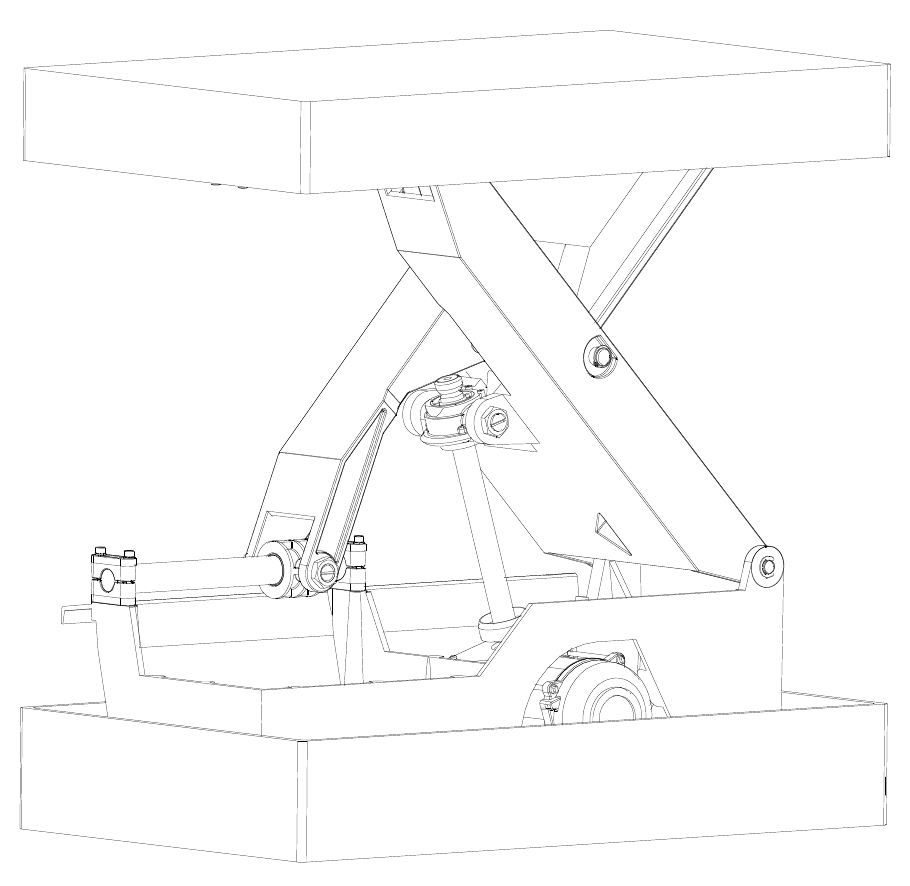
\includegraphics[width=\linewidth]{img/pos_haute.png}
\caption{Position haute}
\label{fig:imagechaise4}
\end{center}
\end{minipage}
\hfill
\begin{minipage}[c]{.4\linewidth}
\begin{center}
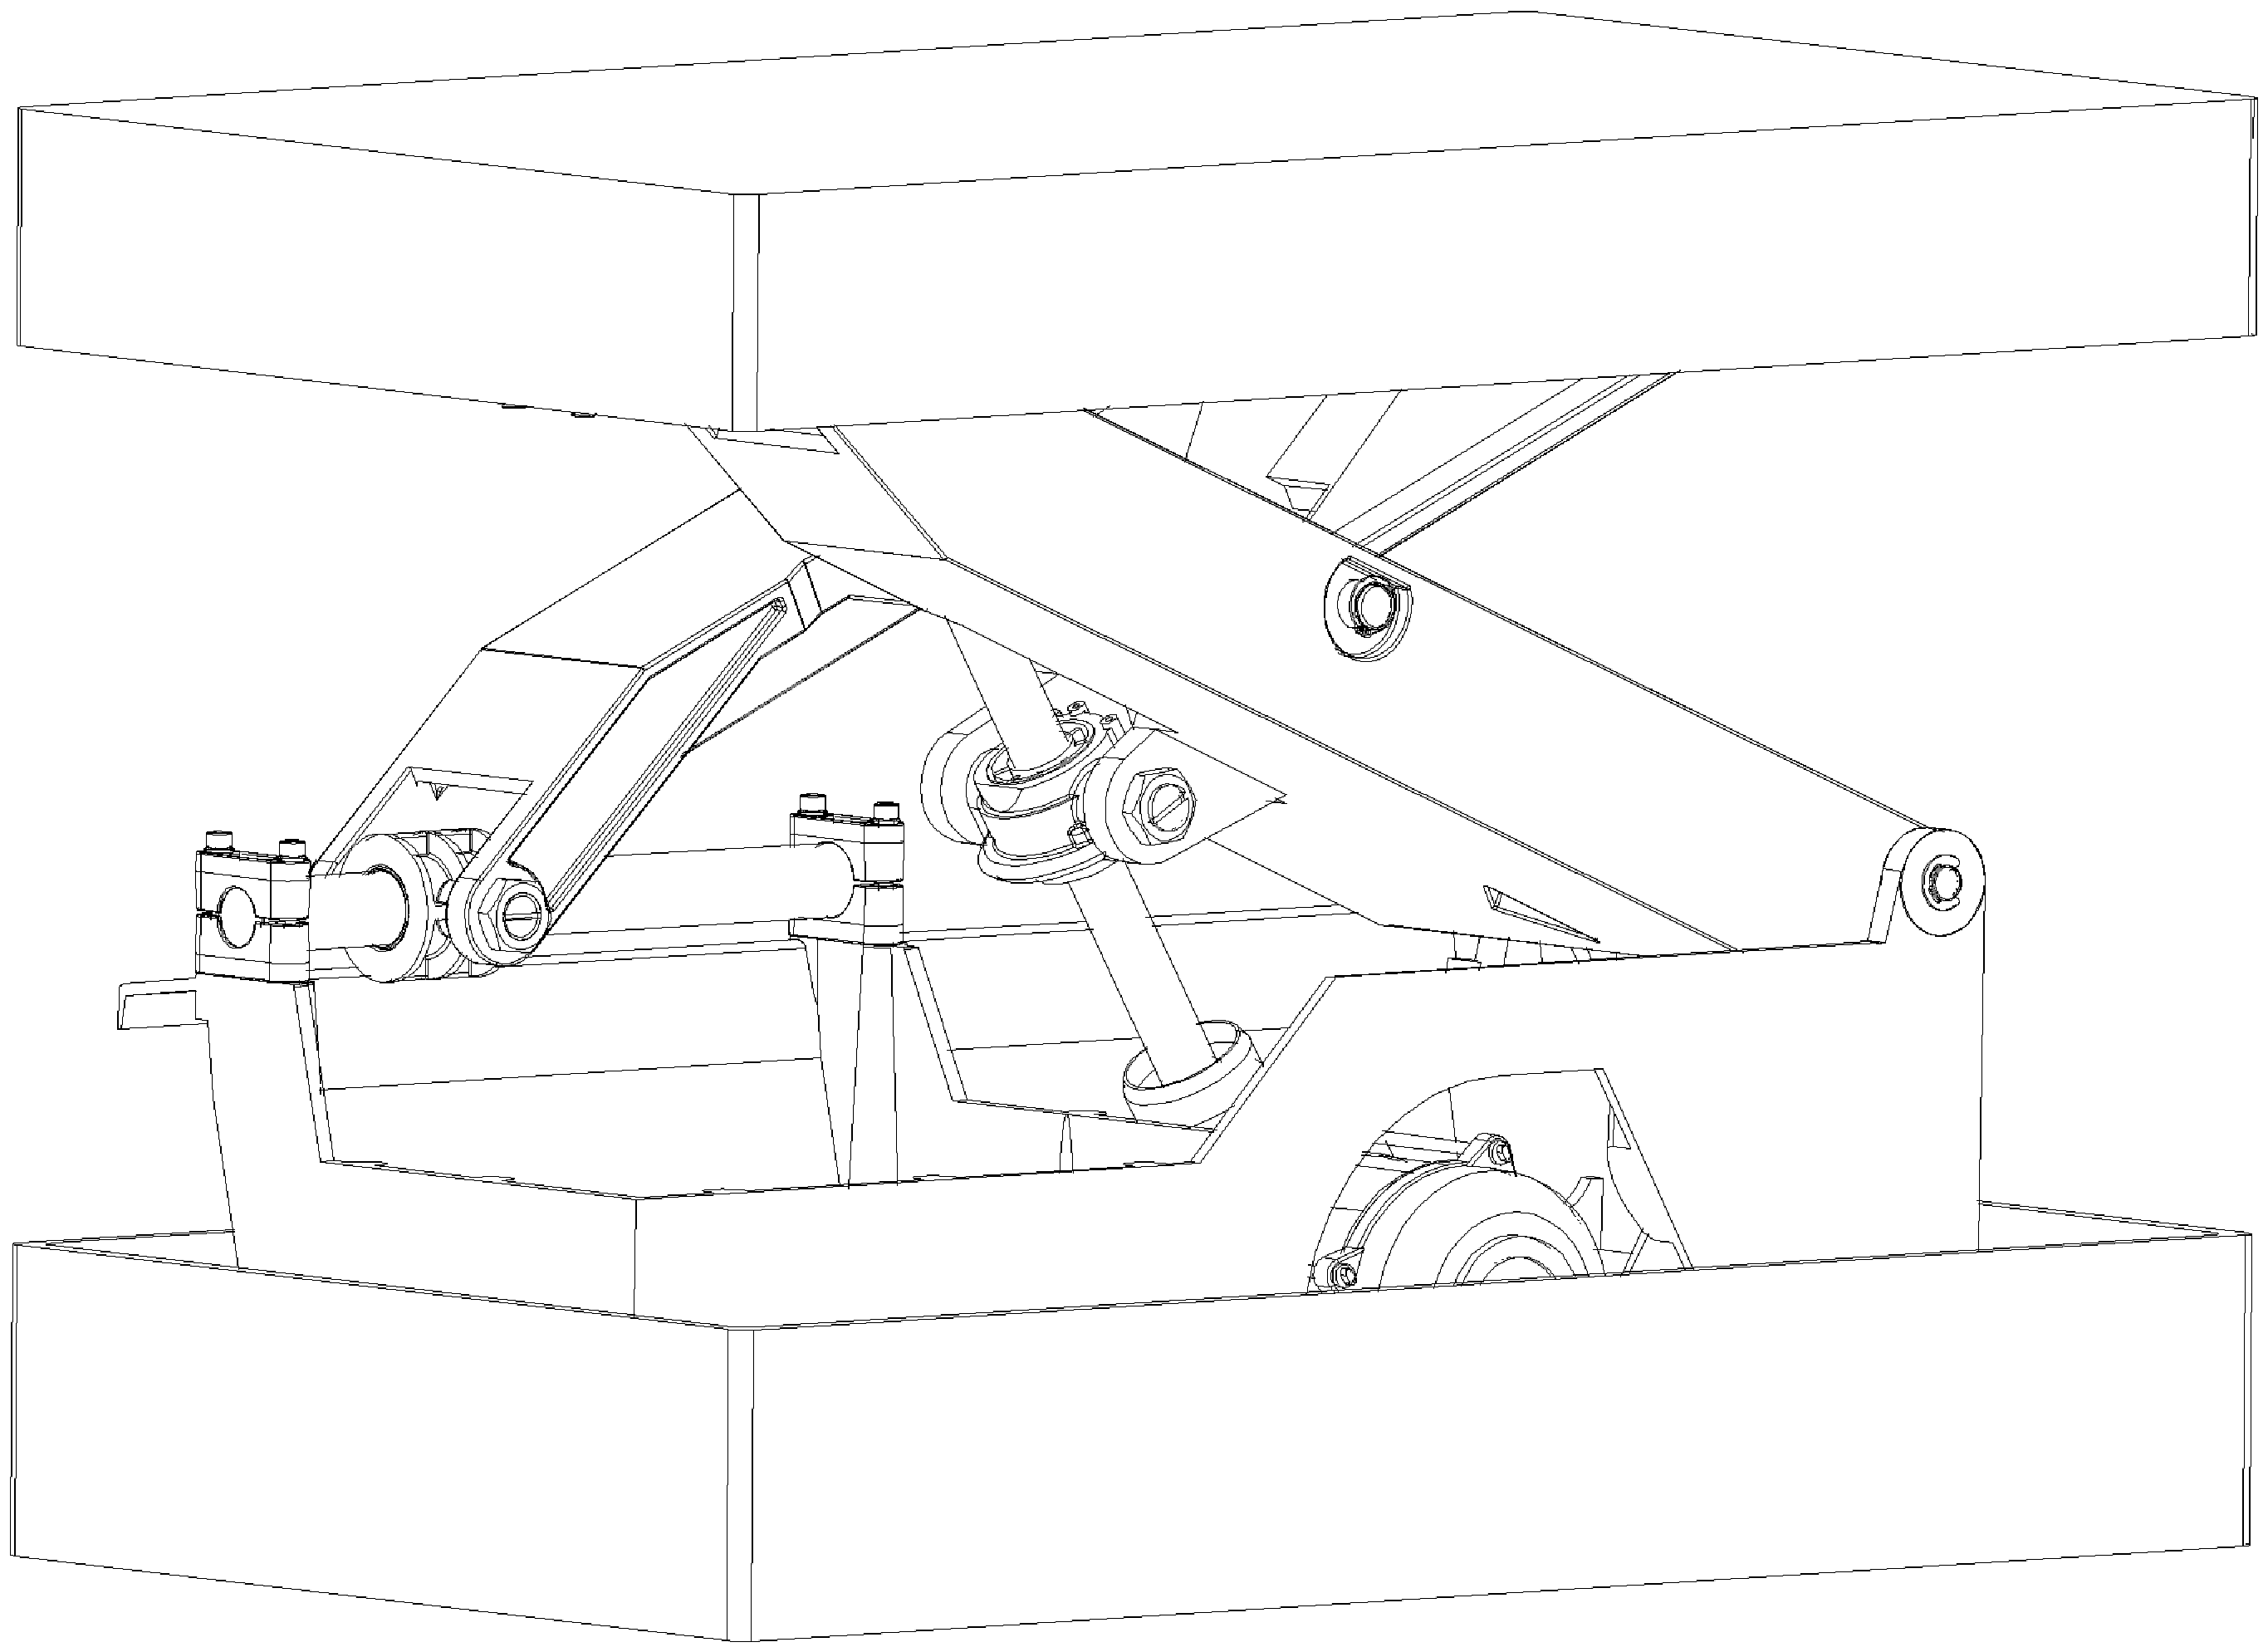
\includegraphics[width=\linewidth]{img/perspective.png}
\caption{Position intermédiaire}
\label{fig:imagechaise5}
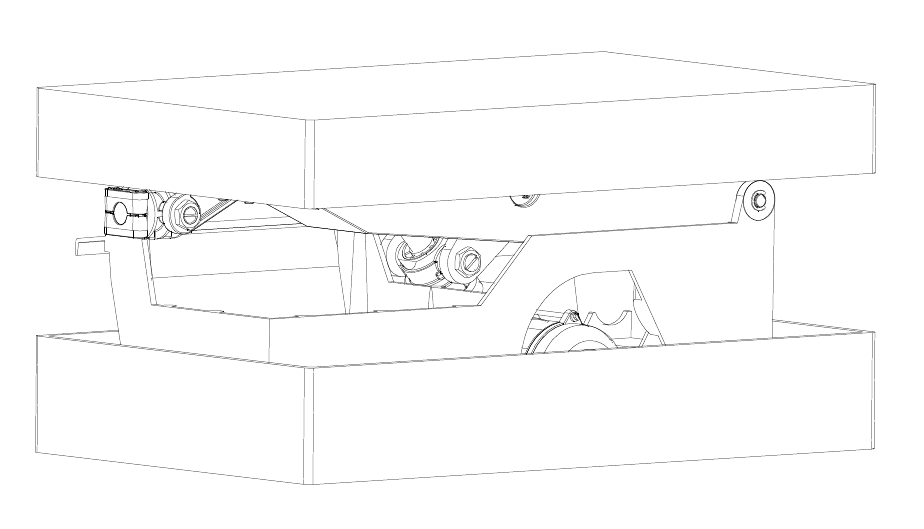
\includegraphics[width=\linewidth]{img/pos_basse.png}
\caption{Position basse}
\label{fig:imagechaise6}
\end{center}
\end{minipage}
\end{figure}

\paragraph{Question 1:} Mettre en place les repères suivants:
\begin{itemize}
 \item $R_6(\overrightarrow{x_6},\overrightarrow{y_6},\overrightarrow{z_6})$ au point A,
 \item $R_3(\overrightarrow{x_3},\overrightarrow{y_3},\overrightarrow{z_3})$ au point D,
 \item $R_4(\overrightarrow{x_4},\overrightarrow{y_4},\overrightarrow{z_4})$ au point H. 
\end{itemize}

\paragraph{Question 2:} Tracer les figures de changement de repère suivantes:
\begin{itemize}
 \item $R_3 \rightarrow R$, angle $\theta_{3}$,
 \item $R_4 \rightarrow R$, angle $\theta_{4}$,
 \item $R_6 \rightarrow R$, angle $\theta_{6}$.
\end{itemize}

\paragraph{Question 3:} Déterminer la relation entre $\theta_{3}$ et $\theta_{4}$.

\paragraph{Question 4:} En utilisant la fermeture géométrique $\overrightarrow{AD}+\overrightarrow{DB}=\overrightarrow{AB}$, définir $l_1$ et $\theta_6$ en fonction de $\theta_3$.

\paragraph{Question 5:} En utilisant une fermeture géométrique déterminer $\theta_3$ en fonction de la longueur $l_2$.

\paragraph{Question 6:} Montrer qu'il est possible de déterminer la position de l'écrou (distance $l_1$) sur l'axe du moteur en fonction de la hauteur du siège (distance $l_2$).

\newpage

\section{Maxpid}

La  chaîne fonctionnelle MAXPID est un sous-ensemble extrait  d'un robot  de  récolte  d'oranges développé par la société PELLENC S.A. de PERTUIS (Vaucluse). 

~\

\begin{wrapfigure}[7]{r}{0.45\textwidth}
  \begin{center}
  \vspace{-1cm}
    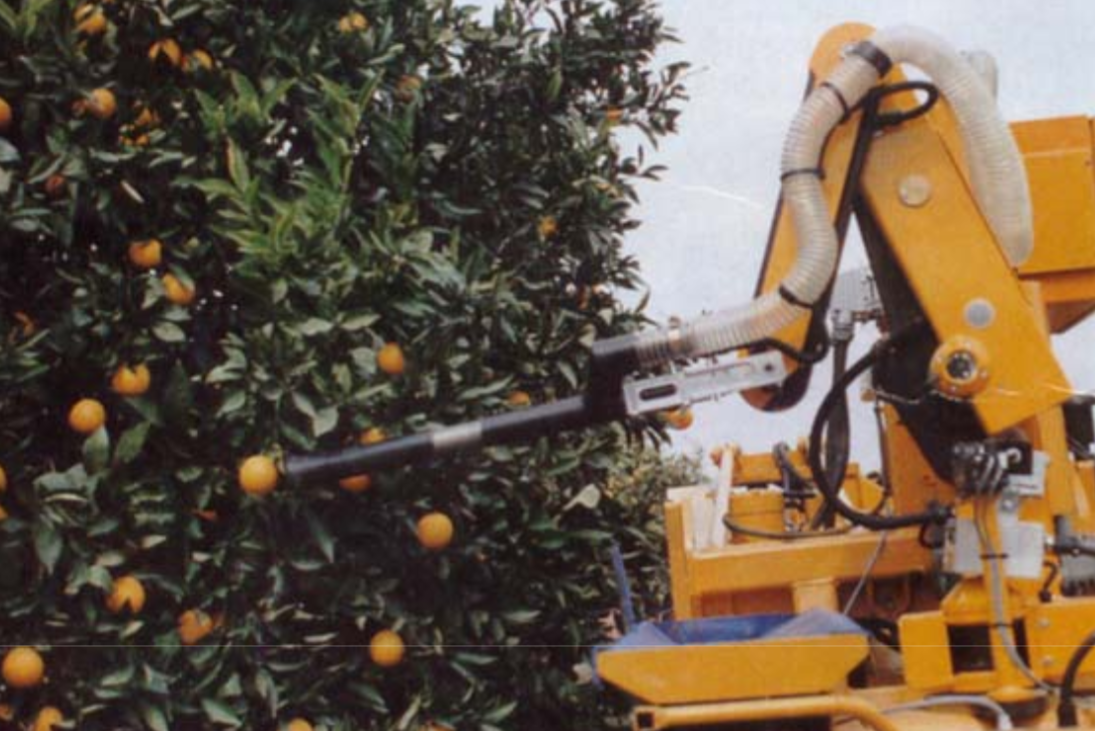
\includegraphics[width=0.7\linewidth]{img/citrus}
  \end{center}
\end{wrapfigure}
Le robot repère et localise automatiquement une orange mûre. Une fois localisée, elle est saisie par une ventouse montée en bout du bras.

La saisie ne sera correcte que si la position du bras est parfaitement contrôlée: le bras doit alors se positionner à l'endroit voulu pour assurer un bon contact de la ventouse et de l'orange. 

~\

Le sous-système Maxpid est représenté sur les figures ci-dessous.

\begin{minipage}{0.5\linewidth}
 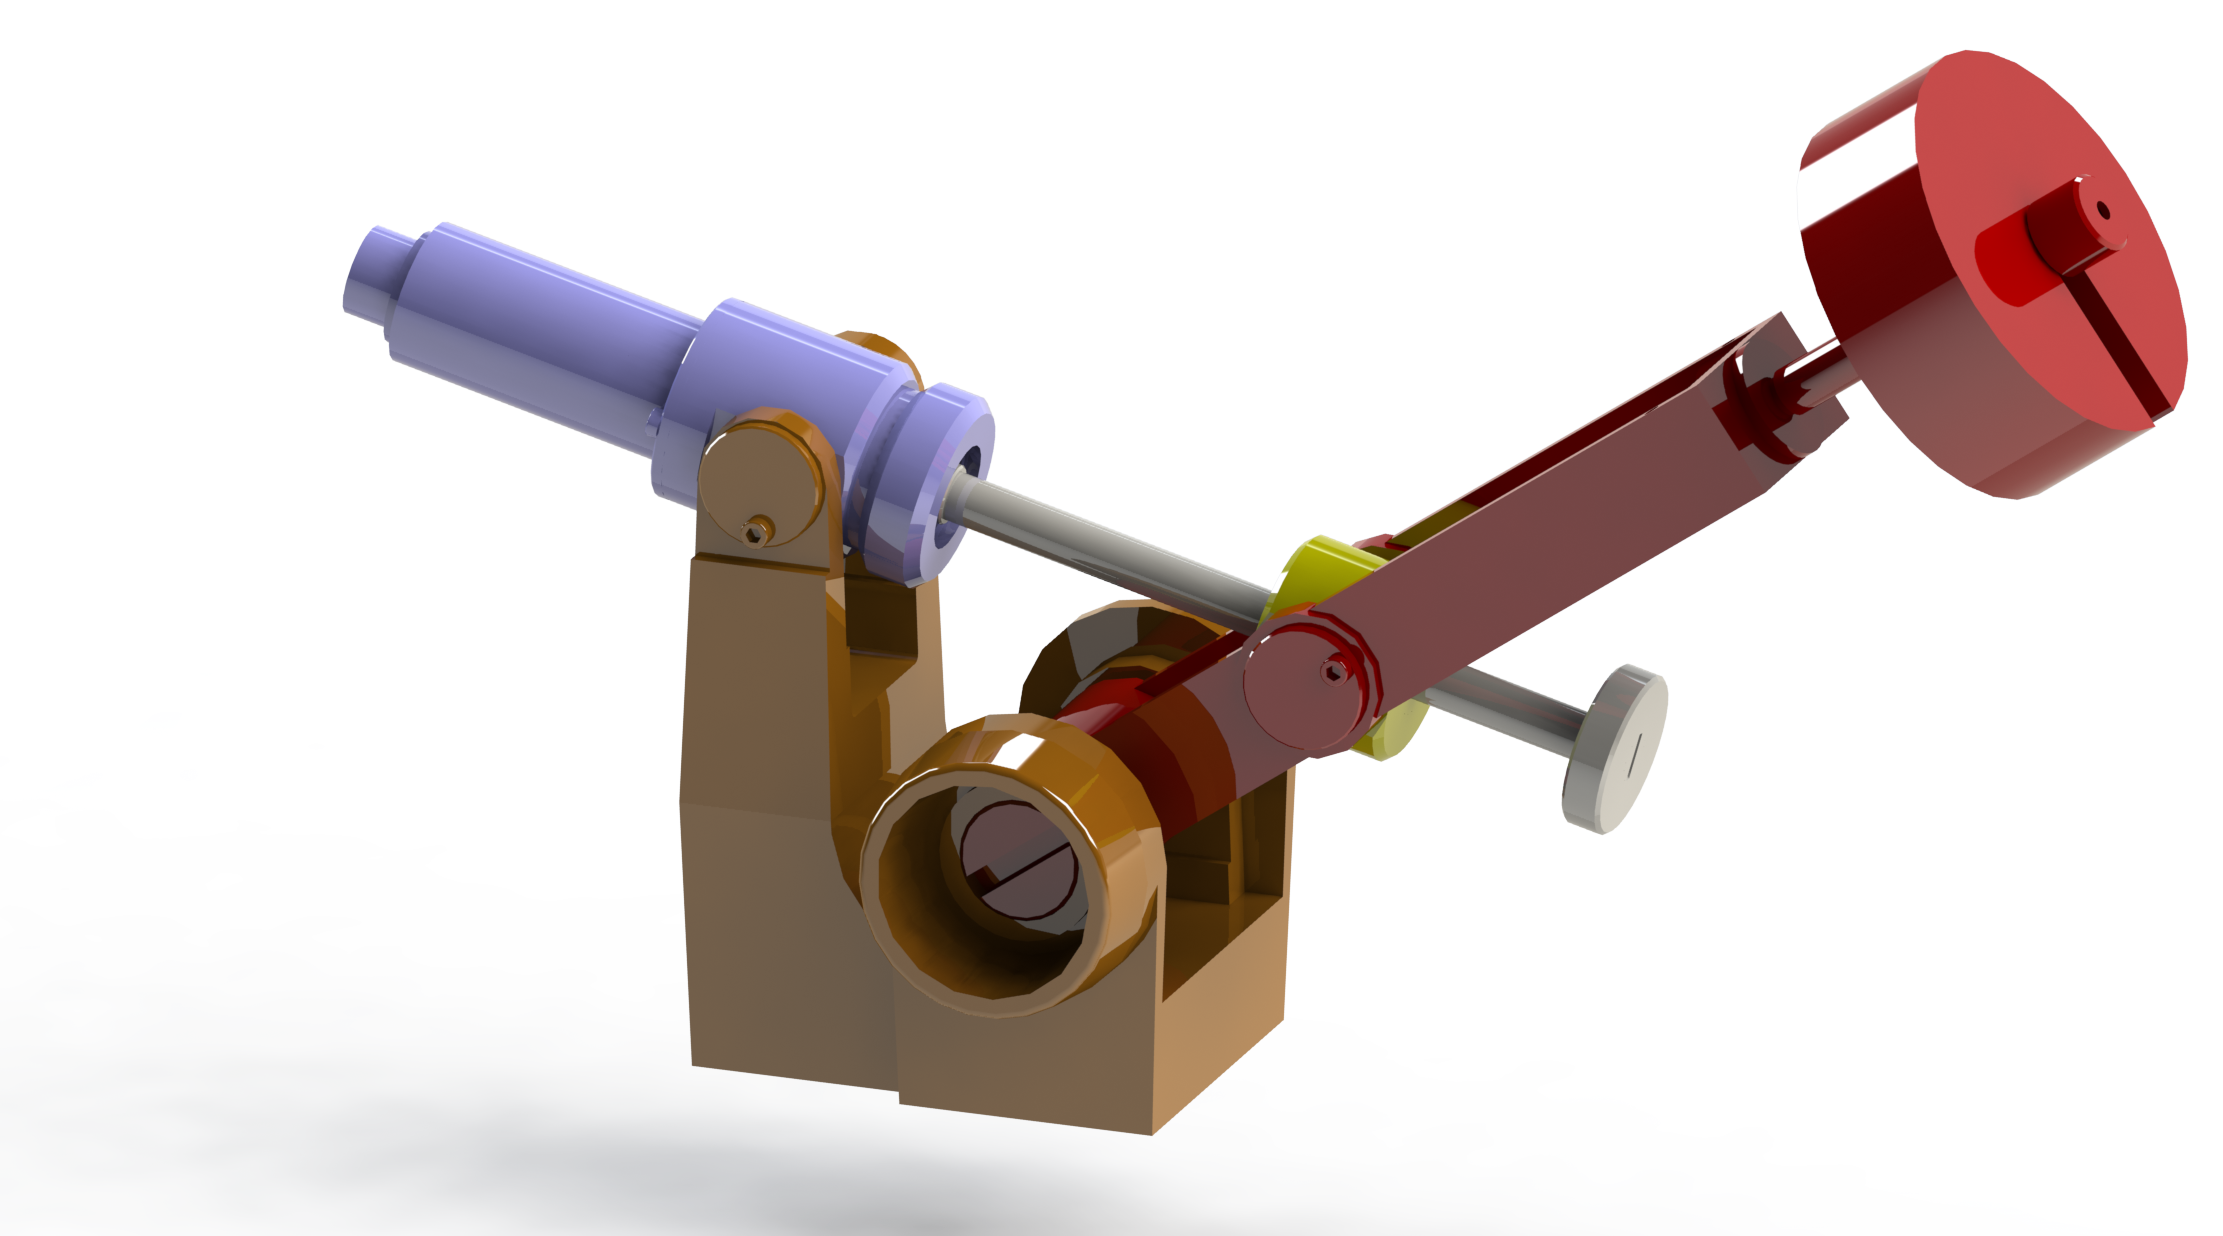
\includegraphics[width=0.9\linewidth]{img/Maxpid3D}
\end{minipage}\hfill
\begin{minipage}{0.45\linewidth}
Pièces du Maxpid:
\begin{enumerate}\setcounter{enumi}{-1}
 \item Chaise,
 \item Bras + masses,
 \item Bâti moteur,
 \item Vis,
 \item Écrou.
\end{enumerate}
\end{minipage}

~\

\begin{center}
	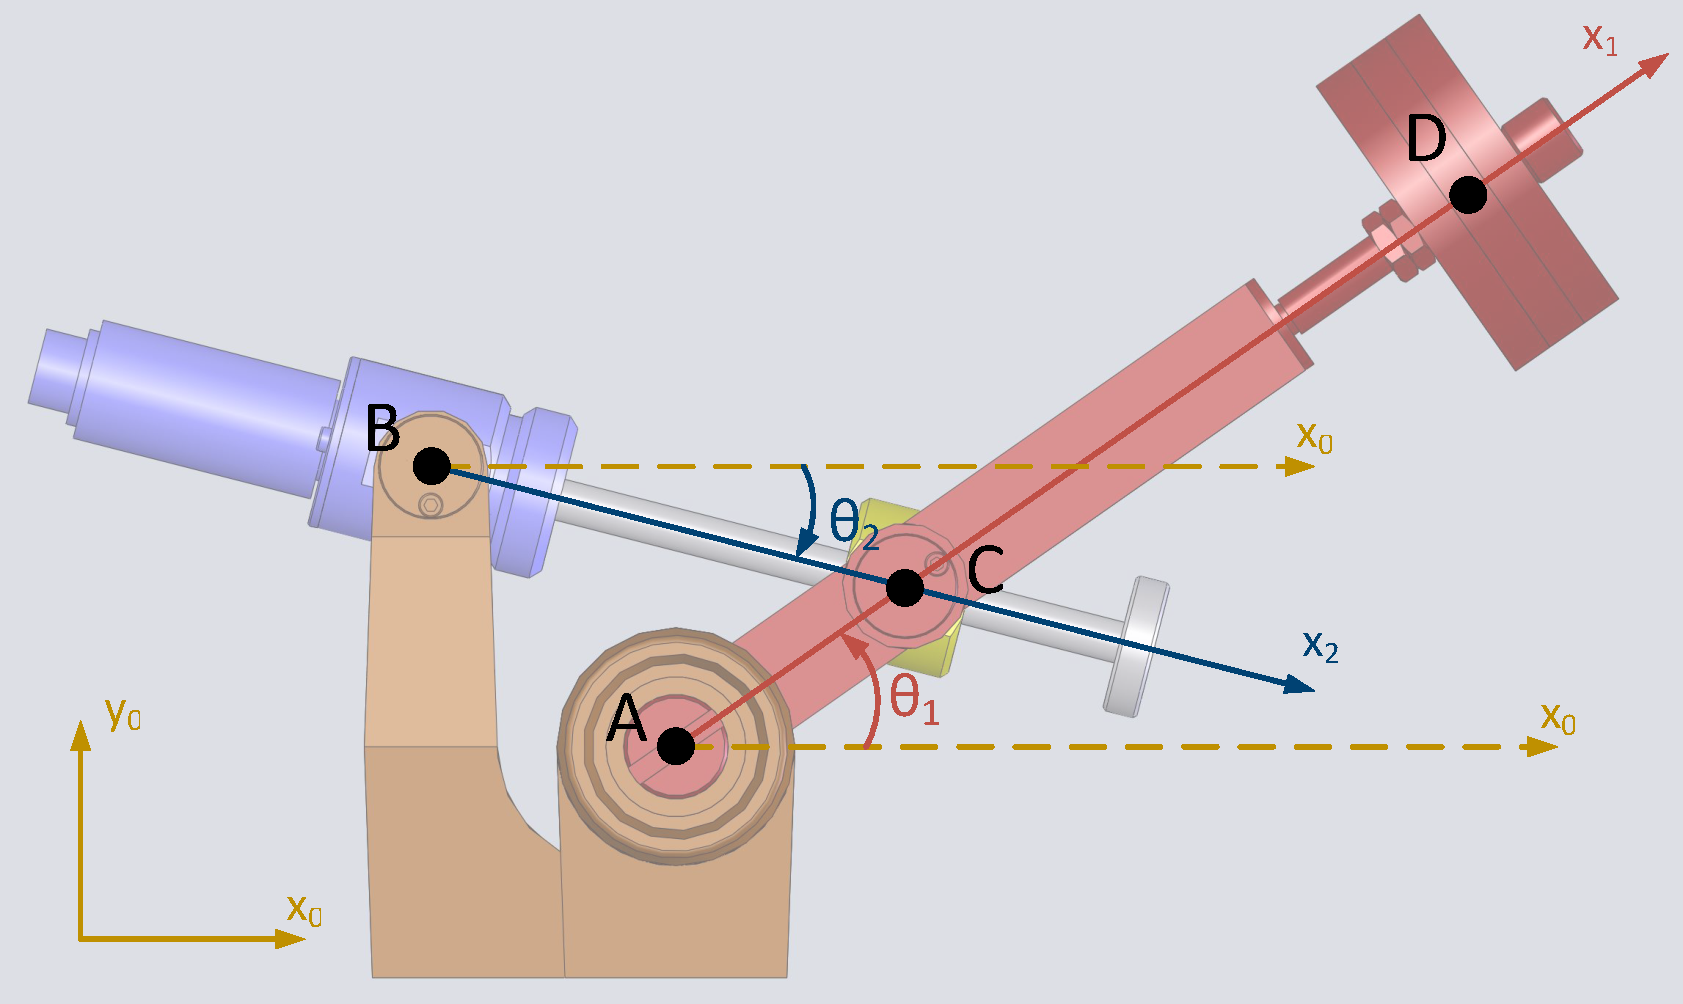
\includegraphics[width=0.9\linewidth]{img/Maxpid_param}
\end{center}


\begin{minipage}{0.45\linewidth}
\begin{itemize}
 \item $\overrightarrow{AB}=-a.\overrightarrow{x_0}+b.\overrightarrow{y_0}$,
 \item $\overrightarrow{BC}=l_1.\overrightarrow{x_2}$,
 \item $\overrightarrow{AC}=c.\overrightarrow{x_1}$. 
\end{itemize}
\end{minipage}\hfill
\begin{minipage}{0.45\linewidth}
Les variables $a$, $b$ et $c$ sont des constantes liées aux dimensions du système. La longueur $l_1$ varie en fonction de la position du système.
\end{minipage}

\paragraph{Question 1:} En utilisant une fermeture géométrique, déterminer $l_1$ en fonction de $\theta_1$ et des dimensions du système.

\paragraph{Question 2:} Montrer que ce résultat peut se mettre sous la forme suivante.

\begin{center}
$l_1^2-a^2-b^2-c^2=X.cos Y.cos\theta_1-X.sin Y.sin\theta_1$
\end{center}

Déterminer $X$ et $Y$ en fonction des dimensions du système.

\paragraph{Question 3:} A partir de cette écriture, déterminer $\theta_1$ en fonction de $l_1$ et des dimensions du mécanisme.

%\newpage

%\begin{figure}[!h]
%	\begin{center}
%	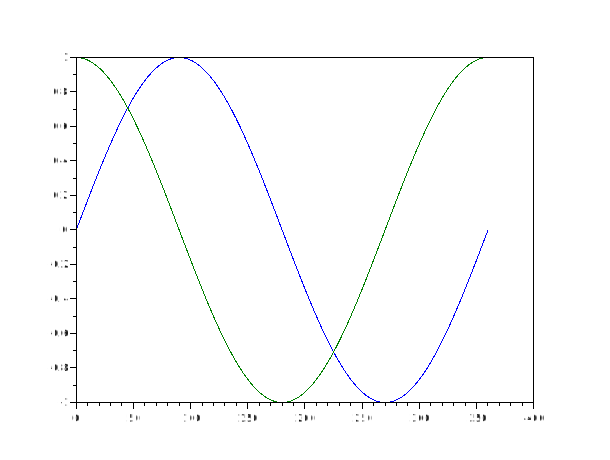
\includegraphics[width=0.7\linewidth]{img/Degres}
%	\end{center}
%	\caption{Cosinus et sinus d'un angle en degrés}
%\end{figure}
%
%\begin{figure}[!h]
%	\begin{center}
%	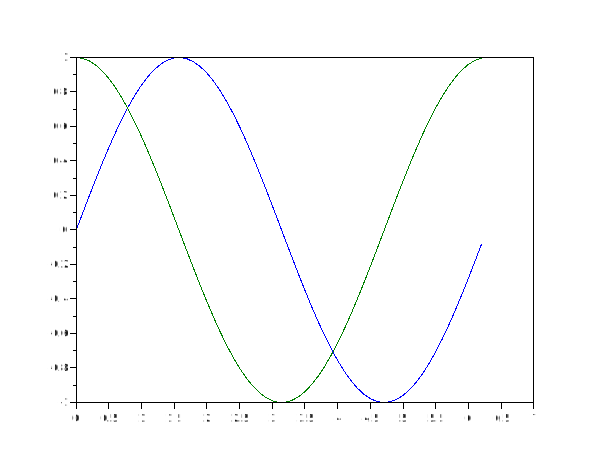
\includegraphics[width=0.7\linewidth]{img/Radians}
%	\end{center}
%	\caption{Cosinus et sinus d'un angle en radians}
%\end{figure}

\ifdef{\public}{\end{document}}

\newpage

\pagestyle{correction}

\section{Correction}

\subsection{Rappels}

\subsubsection{Les bases du produit vectoriel}

\paragraph{Question 1:} La norme du vecteur $\overrightarrow{u}$ est $\|\overrightarrow{u}\|=\sqrt{8^2+5^2+4^2}=10.25$

\paragraph{Question 2:} Si $\overrightarrow{u}$ et $\overrightarrow{v}$ sont colinéaires, alors: 

$\overrightarrow{u}=a.\overrightarrow{v}\rightarrow \left(\begin{array}{c}8 \\ 5 \\ 4 \end{array}\right)=a.\left(\begin{array}{c}6 \\ y \\ z \end{array}\right)=\left(\begin{array}{c} 6a \\ a\times y \\ a\times z \end{array}\right)$

Donc, $a=\frac{8}{6}=\frac{4}{3}$, donc $\left\{\begin{array}{c}y=3.75 \\ z=3 \end{array}\right.$

Si $\overrightarrow{u}$ et $\overrightarrow{v}$ sont colinéaires, par définition: $\overrightarrow{u} \wedge \overrightarrow{v}=\overrightarrow{0}$.

$\left(\begin{array}{c}8 \\ 5 \\ 4 \end{array}\right) \wedge \left(\begin{array}{c}6 \\ y \\ z \end{array}\right)=\left(\begin{array}{c} 5y-4x \\ 24 - 8y \\ 8x-30 \end{array}\right)=\left(\begin{array}{c} 0 \\ 0 \\ 0 \end{array}\right)$.

On retrouve les mêmes résultats.

\subsubsection{Produit scalaire}

\paragraph{Question 1:} $\|\overrightarrow{u}\|=\sqrt{18^2+7^2+13^2}=\sqrt{542}=23.28$

$\|\overrightarrow{v}\|=\sqrt{23^2+54^2+36^2}=\sqrt{4741}=68.85$

\paragraph{Question 2:} $\overrightarrow{u}.\overrightarrow{v}=\left(\begin{array}{c} 18 \\ 7 \\ 13 \end{array}\right).\left(\begin{array}{c} 23 \\ -54 \\ 36 \end{array}\right)=414-378+468=504$

\paragraph{Question 3:} $\|\overrightarrow{u}\|.\|\overrightarrow{v}\|=\sqrt{18^2+7^2+13^2}\times \sqrt{23^2+54^2+36^2}=\sqrt{542}\times \sqrt{4741}=1603$

Donc $cos(\overrightarrow{u},\overrightarrow{v})=\frac{504}{1603}\rightarrow (\overrightarrow{u},\overrightarrow{v})=1.25rad=71.67$\textdegree.

\subsubsection{Produit vectoriel}

\paragraph{Question 1:} $\|\overrightarrow{u}\|=\sqrt{4+9+36}=7$

$\|\overrightarrow{v}\|=\sqrt{1+25+4}=\sqrt{30}=5.48$

\paragraph{Question 2:} $\overrightarrow{u}\wedge \overrightarrow{v}=\left(\begin{array}{c} 2 \\ 3 \\ 6 \end{array}\right)\wedge 
\left(\begin{array}{c} 1 \\ 5 \\ 2 \end{array}\right)=\left(\begin{array}{c} -24 \\ 2 \\ 7 \end{array}\right)$

\paragraph{Question 3:} $\|\overrightarrow{u}\wedge \overrightarrow{v}\|=\sqrt{576+4+49}=\sqrt{629}=25$

$\|\overrightarrow{u}\wedge \overrightarrow{v}\|=\|\overrightarrow{u}\|.\|\overrightarrow{v}\|.sin(\overrightarrow{u},\overrightarrow{v})$

Donc $sin(\overrightarrow{u},\overrightarrow{v})=\frac{7\sqrt{30}}{\sqrt{629}}\rightarrow (\overrightarrow{u},\overrightarrow{v})=0.71rad=40.8$\textdegree.

\newpage

\subsection{Machine de dépose joint}

\paragraph{Question 1:} On nomme ce robot: \og un robot 6 axes \fg car il possède 6 degrés de liberté.

\paragraph{Question 2:}

$\overrightarrow{O_0O_1}=a.\overrightarrow{x_1}+b.\overrightarrow{z_0}-f.\overrightarrow{y_1}=a.\overrightarrow{x_0}+b.\overrightarrow{z_0}-f.\overrightarrow{y_0}$

$\overrightarrow{O_1O_2}=c.\overrightarrow{z_2}$

$\overrightarrow{O_2O_3}=d.\overrightarrow{x_3}+f.\overrightarrow{y_3}=d.\overrightarrow{x_0}+f.\overrightarrow{y_0}$

$\overrightarrow{O_3O_4}=e.\overrightarrow{x_3}+h.\overrightarrow{y_4}=e.\overrightarrow{x_3}+h.\overrightarrow{y_0}$

$\overrightarrow{O_4O_5}=g.\overrightarrow{x_5}=g.\overrightarrow{x_3}$

$\overrightarrow{O_5M}=-h.\overrightarrow{y_6}-l.\overrightarrow{z_6}=-h.\overrightarrow{y_0}-l.\overrightarrow{z_3}$

\paragraph{Question 3:} D'après les figures de changement de repère de la figure \ref{fig:image6}, on constate:

$\left\{\begin{array}{l} \overrightarrow{x_2}=cos(\theta_{12}).\overrightarrow{x_0}-sin(\theta_{12}).\overrightarrow{z_0} \\
\overrightarrow{z_2}=sin(\theta_{12}).\overrightarrow{x_0}+cos(\theta_{12}).\overrightarrow{z_0} \end{array}\right.$

$\left\{\begin{array}{l} \overrightarrow{x_3}=cos(\theta_{12}+\theta_{23}).\overrightarrow{x_0}-sin(\theta_{12}+\theta_{23}).\overrightarrow{z_0} \\
\overrightarrow{z_3}=sin(\theta_{12}+\theta_{23}).\overrightarrow{x_0}+cos(\theta_{12}+\theta_{23}).\overrightarrow{z_0} \end{array}\right.$

Donc,

$\overrightarrow{O_0M}=a.\overrightarrow{x_0}+b.\overrightarrow{z_0}+c.\overrightarrow{z_2}+(d+e+g).\overrightarrow{x_3}-l.\overrightarrow{z_3}$

Enfin,

$\overrightarrow{O_0M}=a.\overrightarrow{x_0}+b.\overrightarrow{z_0}+c.sin(\theta_{12}).\overrightarrow{x_0}+c.cos(\theta_{12}).\overrightarrow{z_0}+(d+e+g).cos(\theta_{12}+\theta_{23}).\overrightarrow{x_0}-(d+e+g)sin(\theta_{12}+\theta_{23}).\overrightarrow{z_0}-l.sin(\theta_{12}+\theta_{23}).\overrightarrow{x_0}-l.cos(\theta_{12}+\theta_{23}).\overrightarrow{z_0}$

\begin{math}
\overrightarrow{O_0M}=\left[a+c.sin(\theta_{12})+(d+e+g).cos(\theta{12}+\theta{23})-l.sin(\theta{12}+\theta{23})\right].\overrightarrow{x_0} \\
+\left[b+c.cos(\theta_{12})-(d+e+g).sin(\theta{12}+\theta{23})-l.cos(\theta{12}+\theta{23})\right].\overrightarrow{z_0}
\end{math}

\subsection{Chaise de dentiste}

\paragraph{Question 1:} Mettre en place les repères suivants:
\begin{itemize}
 \item $R_6(\overrightarrow{x},\overrightarrow{y},\overrightarrow{z})$ au point A,
 \item $R_3(\overrightarrow{x_3},\overrightarrow{y_3},\overrightarrow{z_3})$ au point D,
 \item $R_4(\overrightarrow{x_4},\overrightarrow{y_4},\overrightarrow{z_4})$ au point H. 
\end{itemize}

\paragraph{Question 2:} Tracer les figures de changement de repère suivantes:
\begin{itemize}
 \item $R_3 \rightarrow R$, angle $\theta_{3}$,
 \item $R_4 \rightarrow R$, angle $\theta_{4}$,
 \item $R_6 \rightarrow R$, angle $\theta_{6}$.
\end{itemize}

En déduire les équations vectorielles qui en découlent.

\begin{math}
\left\{\begin{array}{l}
\overrightarrow{x_3}=cos\theta_3.\overrightarrow{x_0}+sin\theta_3.\overrightarrow{y_0}\\
\overrightarrow{y_3}=-sin\theta_3.\overrightarrow{x_0}+cos\theta_3.\overrightarrow{y_0}\\
\overrightarrow{z_3}=\overrightarrow{z_0}
\end{array}\right.
\end{math}

\begin{math}
\left\{\begin{array}{l}
\overrightarrow{x_4}=cos\theta_4.\overrightarrow{x_0}+sin\theta_4.\overrightarrow{y_0}\\
\overrightarrow{y_4}=-sin\theta_4.\overrightarrow{x_0}+cos\theta_4.\overrightarrow{y_0}\\
\overrightarrow{z_4}=\overrightarrow{z_0}
\end{array}\right.
\end{math}

\begin{math}
\left\{\begin{array}{l}
\overrightarrow{x_6}=cos\theta_6.\overrightarrow{x_0}+sin\theta_6.\overrightarrow{y_0}\\
\overrightarrow{y_6}=-sin\theta_6.\overrightarrow{x_0}+cos\theta_6.\overrightarrow{y_0}\\
\overrightarrow{z_6}=\overrightarrow{z_0}
\end{array}\right.
\end{math}

\paragraph{Question 3:} Déterminer la relation entre $\theta_{3}$ et $\theta_{4}$.

$\overrightarrow{DE}.\overrightarrow{x}=0=(\overrightarrow{DC}+\overrightarrow{CE}).\overrightarrow{x}=(c.\overrightarrow{x_3}+c.\overrightarrow{x_4}).\overrightarrow{x}$

Donc, $c.cos\theta_3+c.cos\theta_4=0$, donc $cos\theta_3=-cos\theta_4$, donc $\theta_3=\pi-\theta_4$.

\paragraph{Question 4:} En utilisant la fermeture géométrique $\overrightarrow{AD}+\overrightarrow{DB}=\overrightarrow{AB}$, définir $l_1$ et $\theta_6$ en fonction de $\theta_3$.

$\overrightarrow{AD}+\overrightarrow{DB}=\overrightarrow{AB}$
$a.\overrightarrow{x}+b.\overrightarrow{y}+d.\overrightarrow{x_3}+e.\overrightarrow{y_3}=l_1.\overrightarrow{x_6}$

$a.\overrightarrow{x}+b.\overrightarrow{y}+d.cos\theta_3.\overrightarrow{x}+d.sin\theta_3.\overrightarrow{y}-e.sin\theta_3.\overrightarrow{x}+e.cos\theta_3.\overrightarrow{y}=l_1.cos\theta_6.\overrightarrow{x}+l_1.sin\theta_6.\overrightarrow{y}$

\begin{math}
\left\{\begin{array}{l}
a+d.cos\theta_3-e.sin\theta_3=l_1.cos\theta_6\\
b+d.sin\theta_3+e.cos\theta_3=l_1.sin\theta_6
\end{array}\right.
\end{math}

~\

Calcul de $l_1$:

$(a+d.cos\theta_3-e.sin\theta_3)^2+(b+d.sin\theta_3+e.cos\theta_3)^2=(l_1.cos\theta_6)^2+(l_1.sin\theta_6)^2$

Donc, $l_1=\sqrt{(a+d.cos\theta_3-e.sin\theta_3)^2+(b+d.sin\theta_3+e.cos\theta_3)^2}$.

~\

Calcul de $\theta_6$:

$\dfrac{b+d.sin\theta_3+e.cos\theta_3}{a+d.cos\theta_3-e.sin\theta_3}=\dfrac{l_1.sin\theta_6}{l_1.cos\theta_6}$

Donc, $\theta_6=arctan\left(\dfrac{b+d.sin\theta_3+e.cos\theta_3}{a+d.cos\theta_3-e.sin\theta_3}\right)$.

\paragraph{Question 5:} En utilisant une fermeture géométrique déterminer $\theta_3$ en fonction de la longueur $l_2$.

$\overrightarrow{DE}=\overrightarrow{DC}+\overrightarrow{CE}$
$l_2.\overrightarrow{y}=c.\overrightarrow{x_3}+c.\overrightarrow{x_4}$

$l_2=c.sin\theta_3+c.sin\theta_4$, avec $\theta_4=\pi-\theta_3$, donc

$l_2=2.c.sin\theta_3$, donc $\theta_3=arcsin\left(\frac{l_2}{2.c}\right)$

\paragraph{Question 6:} Montrer qu'il est possible de déterminer la position de l'écrou (distance $l_1$) sur l'axe du moteur en fonction de la hauteur du siège (distance $l_2$).

Bilan des équations:
\begin{math}
\left\{\begin{array}{l}
\theta_3=arcsin\left(\frac{l_2}{2.c}\right)\\
l_1=\sqrt{(a+d.cos\theta_3-e.sin\theta_3)^2+(b+d.sin\theta_3+e.cos\theta_3)^2}\\
\theta_6=arctan\left(\dfrac{b+d.sin\theta_3+e.cos\theta_3}{a+d.cos\theta_3-e.sin\theta_3}\right)
\end{array}\right.
\end{math}

L'équation 1 permet de déterminer $\theta_3$ en fonction de $l_2$ et l'équation 2 permet de déterminer $l_1$ en fonction de $\theta_3$. Il est donc possible de déterminer $l_2$ en fonction de $l_1$.

\subsection{Maxpid}

\paragraph{Question 1:} En utilisant une fermeture géométrique, déterminer $l_1$ en fonction de $\theta_1$ et des dimensions du système.

$\overrightarrow{AB}+\overrightarrow{BC}=\overrightarrow{AC}$

$-a.\overrightarrow{x_0}+b.\overrightarrow{y_0}+l_1.\overrightarrow{x_2}=c.\overrightarrow{x_1}$

$-a.\overrightarrow{x_0}+b.\overrightarrow{y_0}+l_1.cos\theta_2.\overrightarrow{x_0}+l_1.sin\theta_2\overrightarrow{y_0}=c.cos\theta_1.\overrightarrow{x_0}+c.sin\theta_1.\overrightarrow{y_0}$

\begin{math}
\left\{
\begin{array}{l}
-a+l_1.cos\theta_2=c.cos\theta_1\\
b+l_1.sin\theta_2=c.sin\theta_1
\end{array}\right.
\end{math}

$l_1^2=(c.cos\theta_1+a)^2+(c.sin\theta_1-b)^2$

\paragraph{Question 2:} Montrer que ce résultat peut se mettre sous la forme: $l_1^2-a^2-b^2-c^2=X.cos Y.cos\theta_1-X.sin Y.sin\theta_1$. Déterminer $X$ et $Y$ en fonction des dimensions du système.

$l_1^2=(c.cos\theta_1)^2+a^2+2.a.c.cos\theta_1+(c.sin\theta_1)^2+b^2-2.b.c.sin\theta_1$

$l_1^2-a^2-b^2-c^2=2.a.c.cos\theta_1-2.b.c.sin\theta_1$

$l_1^2-a^2-b^2-c^2=X.cos Y.cos\theta_1-X.sin Y.sin\theta_1$

On peut écrire:
\begin{math}
\left\{
\begin{array}{l}
X.cos Y=2.a.c\\
X.sin Y=2.b.c
\end{array}\right.
\end{math}

\begin{math}
\left\{
\begin{array}{l}
X=2.c.\sqrt{a^2+b^2}\\
Y=arctan\left(\frac{b}{a}\right)
\end{array}\right.
\end{math}

\paragraph{Question 3:} A partir de cette écriture, déterminer $\theta_1$ en fonction de $l_1$ et des dimensions du mécanisme.

$l_1^2-a^2-b^2-c^2=X.cos(\theta_1+Y)$

$\theta_1=arccos\left(\frac{l_1^2-a^2-b^2-c^2}{X}\right)-Y$

$\theta_1=arccos\left(\frac{l_1^2-a^2-b^2-c^2}{2.c.\sqrt{a^2+b^2}}\right)-arctan\left(\frac{b}{a}\right)$

\end{document}
